\documentclass[11 pt]{article}
\usepackage{graphicx}
\usepackage{tikz}
\usetikzlibrary{automata, positioning, arrows}
\usepackage[export]{adjustbox}
\usepackage{float}
\usepackage{amsmath}
\usepackage{pgfplots}
\pgfplotsset{compat=1.15}
\title{EE348 Homework 1}
\date{2018\\ April}
\author{Nail Tosun - 2094563 \\ Electric and Electronic Engineering Department, METU}
\begin{document}
\maketitle
\section*{Question 1}
\subsection*{Part a}
\begin{figure}[H]
\centering
  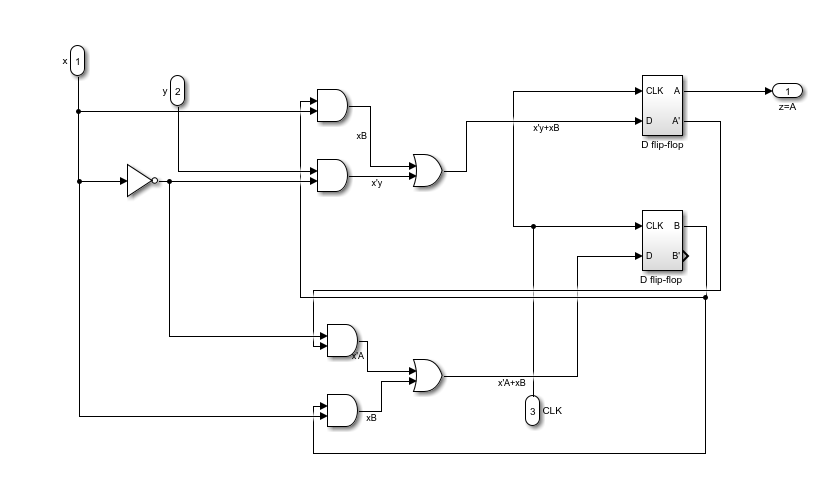
\includegraphics[scale=0.7]{q1}
  \caption{Logic diagram of the circuit}
  \label{fig:zero}
\end{figure}
\subsection*{Part b}
\begin{figure}[H]
\centering
  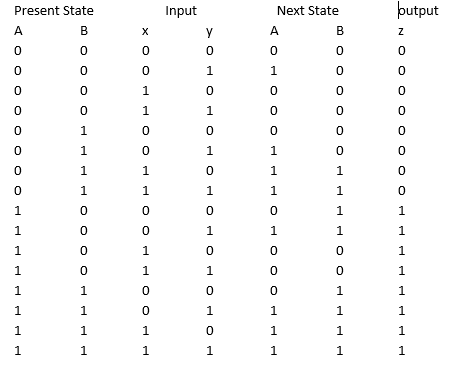
\includegraphics[scale=0.7]{q1_2}
  \caption{State Table}
  \label{fig:zero}
\end{figure}
\subsection*{Part c}
\newpage

\section*{Question 2}
\subsection*{Part a}
\begin{figure}[H]
\centering
  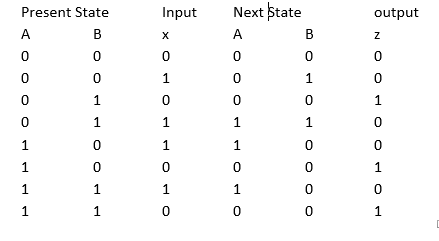
\includegraphics[scale=0.7]{q2}
  \caption{State table of the logic circuit}
  \label{fig:zero}
\end{figure}

\subsection*{Part b}
\begin{figure}[H]
\centering
  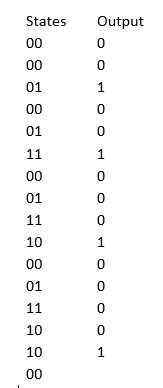
\includegraphics[scale=0.7]{q2_'}
  \caption{States and output of the logic circuit}
  \label{fig:zero}
\end{figure}
\section*{Question 3}
\[A(n+1)=(A+B)\mathbin{\oplus} A = A'B\]
\[B(n+1)=(A'+B)\mathbin{\oplus} B = A'B'\]
\begin{figure}[H]
\centering
  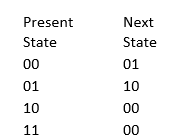
\includegraphics[scale=0.7]{q3}
  \caption{State table of the logic circuit}
  \label{fig:zero}
\end{figure}
When  we look at the state diagram i saw that circuit is 0 to 2 counter. 
\section*{Question 4}
\begin{figure}[H]
\centering
  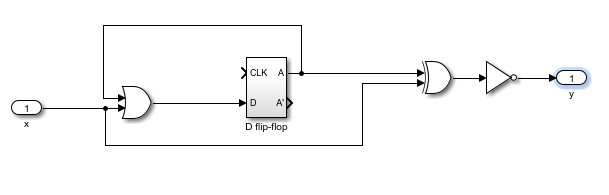
\includegraphics[scale=0.7]{q4}
  \caption{Design of 2's complementer}
  \label{fig:zero}
\end{figure}
Calculations are in appendix.
\section*{Question 5}
\begin{figure}[H]
\centering
  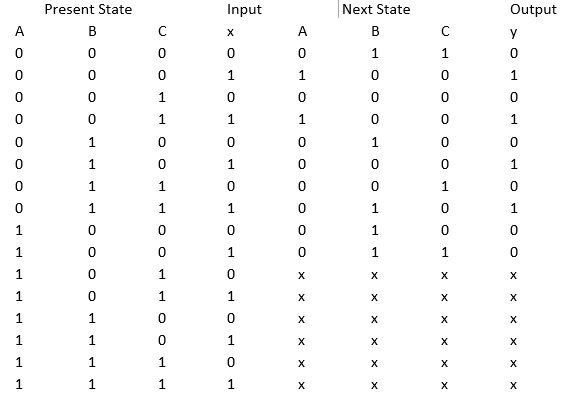
\includegraphics[scale=0.7]{q5}
  \caption{State table of the state diagram}
  \label{fig:zero}
\end{figure}
$$T_{mech}=\frac{N_{ph}I_2^2R_2N_{poles}}{s 4 \pi }$$

\end{document}